\documentclass{article} % For LaTeX2e
\usepackage{nips15submit_e,times}
\usepackage{hyperref}
\usepackage{url}
\usepackage{graphicx}
\usepackage{float}
\usepackage{amsmath}
\usepackage{multirow,array}
\usepackage{listings}
\usepackage{amsfonts}
\usepackage{caption}
\usepackage{subfigure}
\usepackage{algorithm,algorithmic}

%\documentstyle[nips14submit_09,times,art10]{article} % For LaTeX 2.09
%\usepackage{fontspec}

\renewcommand{\algorithmicrequire}{ \textbf{Input:}} %Use Input in the format of Algorithm
\renewcommand{\algorithmicensure}{ \textbf{Output:}} %UseOutput in the format of Algorithm

\definecolor{mygreen}{rgb}{0,0.6,0}
\definecolor{mygray}{rgb}{0.5,0.5,0.5}
\definecolor{mymauve}{rgb}{0.58,0,0.82}
\lstset{ %
backgroundcolor=\color{white},   % choose the background color
basicstyle=\footnotesize\ttfamily,        % size of fonts used for the code
columns=fullflexible,
breaklines=true,                 % automatic line breaking only at whitespace
captionpos=b,                    % sets the caption-position to bottom
tabsize=4,
commentstyle=\color{mygreen},    % comment style
escapeinside={\%*}{*)},          % if you want to add LaTeX within your code
keywordstyle=\color{blue},       % keyword style
stringstyle=\color{mymauve}\ttfamily,     % string literal style
frame=single,
rulesepcolor=\color{red!20!green!20!blue!20},
% identifierstyle=\color{red},
language=python,
numbers=left
}

\title{Weekly Report(May 7 - May 13)}


\author{
Liu Junnan
}

% The \author macro works with any number of authors. There are two commands
% used to separate the names and addresses of multiple authors: \And and \AND.
%
% Using \And between authors leaves it to \LaTeX{} to determine where to break
% the lines. Using \AND forces a linebreak at that point. So, if \LaTeX{}
% puts 3 of 4 authors names on the first line, and the last on the second
% line, try using \AND instead of \And before the third author name.

\newcommand{\fix}{\marginpar{FIX}}
\newcommand{\new}{\marginpar{NEW}}

%\nipsfinalcopy % Uncomment for camera-ready version

\begin{document}


\maketitle

\begin{abstract}
This week I went on cs231n course and started to do assignment 2.
\end{abstract}

\section{Work Done}
\subsection{Convolutional Network}
Convolutional neural networks play a critical role in computer vision domain, because they improve the performance of almost all the CV tasks compared to traditional "shallow" machine learning methods. A typical convnet consists of a series of repeated conv-ReLU layers and fully connected layers in the end. Because the input of CV problems, which are mostly images, have three dimensions of width, height and depth(RGB channels), a convolutional layer takes a 3d matrix as input and also yields a 3d matrix with the same depth of input. A conv layer has multiple filters, each of which convolves the input image, that is, slides over image spatially and computes dot products(imaging the 3d matrices are unraveled as 1d vectors. Actually the dot product of unraveled vectors is mathematically equal to the convolution operation of 3d matrices). A filter convolving the images produces a 2d matrix, and all the output of filters stacked along depth dimension produces the output of this convolutional layer.

\begin{figure}[H]
    \centering
    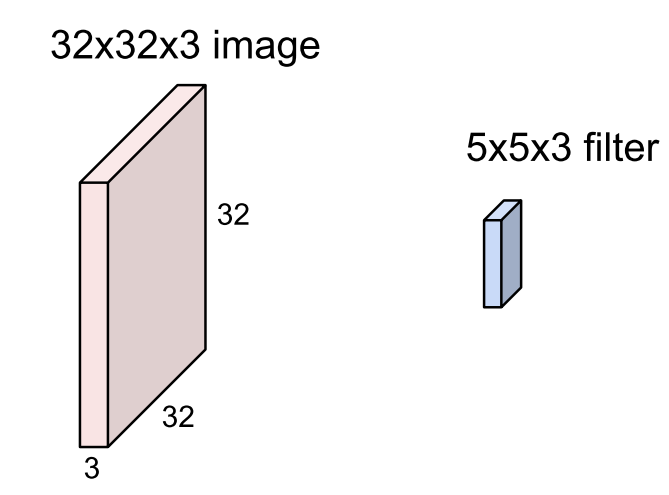
\includegraphics[width=.4\textwidth]{convlayer.png}
    \label{fig:convlayer}
    \caption{Example of convolutional Layer(with one filter)}
\end{figure}

Pooling layers are sometime used right after conv-relu layers to squeeze the spatial size(height and width) of flowing tensors to lower the number of learnable weights of the remaining layers. 
\begin{figure}[H]
    \centering
    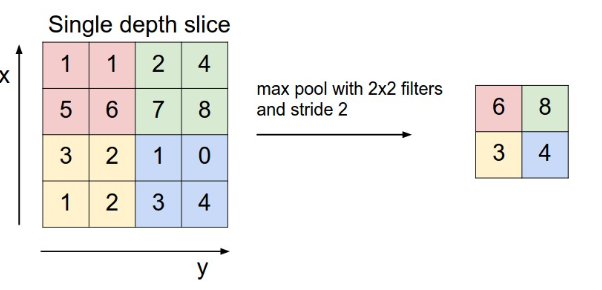
\includegraphics[width=.5\textwidth]{poolinglayer.png}
    \label{fig:poolinglayer}
    \caption{Example of pooling layer}
\end{figure}

There are plenty of details regarding to the implementation of convnet, and I will leave them to the assignment part of next report.

\subsection{Batch Normalization}
Batch Normalization was proposed by Ioffe et al in 2015. The intuition is that if the distribution of each layer is gaussian, the training will be much easier. The equation of normalization is given as $$\hat{x}=\frac{x-E[x]}{\sqrt{Var[x]}}$$
Note that the expectation and variance are based on the mini-batch, which is why the method is named batch normalization.

Another issue is that simply normalizing each input of a layer may change what the layer can represent. This paper suggests that for each activation $x^{(k)}$, we add a pair of parameters $\gamma^{(k)}$, $\beta^{(k)}$, which scale and shift the normalized value:
$$y^{(k)}=\gamma^{(k)} * \hat{x}^{(k)} + \beta^{(k)}$$
These parameters are learned along with the original model parameters, and restore the representation power of the network.

Computing the gradients is not difficult since all the equations are differentiable. One thing needs be noticed that batch normalization layer behaves different during training and testing. During test time, the expectation and variance are estimated by all the training data instead of mini-batch.

\subsection{Installing PyTorch}
The instructor of cs231n introduced TensorFlow and PyTorch as preferred deep learning frameworks. TensorFlow provides a useful visualization tool called TensorBoard that can visualize your network architecture and monitor the process of training. But on the other hand the code is a little bit hard to write, since we have to first create a symbolic graph without actual computation, and then starts the computations that use another set of APIs, which I think will take quite a lot time to learn and get familiar to the APIs.  So I decide to use PyTorch instead.

My laptop has Win10 OS and a CUDA compatible GPU, so I installed Win10-CUDA-enabled version of PyTorch via Anaconda following the installation instruction on PyTorch website, which goes quite smooth. Then I downloaded and installed CUDA9.1 from NVIDIA website. Enabling GPU computation on PyTorch is quite simple, you just have to move the variables to GPU and everything else is done automatically by PyTorch.

\subsection{Assignment 2}
I finished assignment 1 last week so I started assignment 2 this week since their contents are continuous. The implementation of 2- layered fully-connected neural network has done in assignment 1, but the code is imperative, non-modular-style, which is not scalable and extended to the case of multi-layer neural networks. Thus assignment 2 abstracts forward and backward process of layers and implement a feed forward neural network in a more modular approach. In my opinion, I prefer the modular philosophy.

\subsubsection{FC Net}
A fully-connected takes $x$(the input matrix), $w$(weights), $b$(bias) as input, and computes dot product as output. The input matrices are sometime multiple dimensional($> 2$), which means each example has more than 1 dimension. For example the input $x$ has shape $(N, d_1, ..., d_k)$ and contains a minibatch of $N$ examples, where each example $x[i]$ has shape $(d_1, ..., d_k)$. So it is more efficient to reshape each input into a matrix of dimension $D=\prod_{i=1}^k d_i$ and then compute the dot products. Therefore FC layer is also called affine layer. The forward pass is simple:
\begin{lstlisting}
x_flat = x.reshape((N, -1))
out = x_flat.dot(w) + b
cache = (x, w, b)
return out, cache
\end{lstlisting}
Notice that there is an extra variable cache, and it will be returned by the forward pass of all kinds of layers. The reason is that it will be more convenient for backward pass to compute gradients.

The backward pass is also naive:
\begin{lstlisting}
x_flat = x.reshape((N, -1))
dw = x_flat.T.dot(dout)
dx = dout.dot(w.T).reshape(x.shape)
db = dout.sum(0)
\end{lstlisting}
The softmax loss is identical to the one we've implemented in the previous assignment.

Now all the components, except SGD-based optimizers, of a multi-layered fully-connected neural network are done. The test shows the implementation is correct.

\subsubsection{Update Rules}
Vanilla SGD has already been implemented in assignment 1, and this assignment requires us to implement SGD+Momentum, RMSProp and Adam. Although the math behind them is complicated, the code is not. Follow the equation and the implementation is straightforward.

\subsubsection{BatchNorm}
Assignment 2 uses another approach in test time compared to the original averaging method. During training we keep an exponentially decaying running mean of the mean and variance of each feature, and these averages are used to normalize data at test-time.

At each timestep we update the running averages for mean and variance using an exponential decay based on the momentum parameter:

running\_mean = momentum * running\_mean + (1 - momentum) * sample\_mean
    
running\_var = momentum * running\_var + (1 - momentum) * sample\_var

After the code of BatchNorm layer is finished, we insert them to the fully-connected network, and compare the training time compared to the net without BatchNorm. Here is the result
\begin{figure}[H]
  \centering
  % Requires \usepackage{graphicx}
  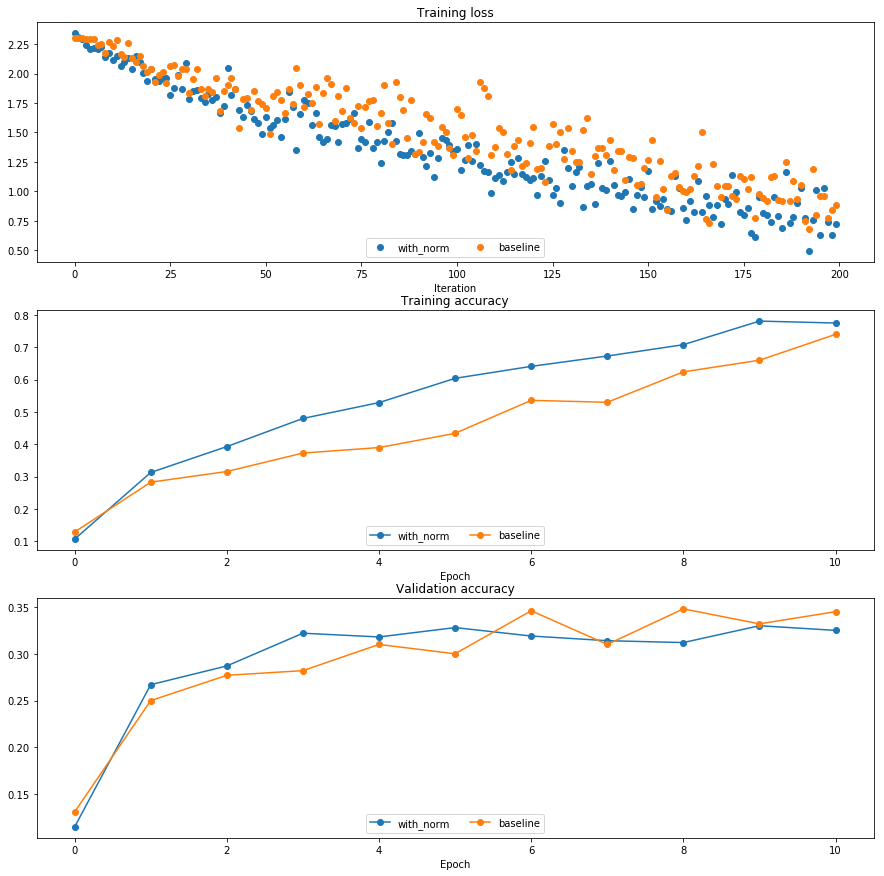
\includegraphics[width=.8\textwidth]{batchnorm.png}\\
  \caption{Training speedup}\label{fig:batchnorm}
\end{figure}

This simple experiment shows that the validation accuracies are comparable, but FC net with batch norm is much faster than baseline(without batch norm). It can be expected that FC with batch norm will exceed FC without batch norm given the same training time.

\section{Plans}
In the next week I plan to finish assignment 2 and continue to learn cs231n course.

\end{document}
